\documentclass[10pt]{article}
\usepackage[margin=0.69in]{geometry}
\usepackage{amsmath,amssymb,graphicx,xcolor,hyperref}
\usepackage{enumitem}
\setlength{\parindent}{0pt}\setlength{\parskip}{6pt}
\hypersetup{colorlinks=true,urlcolor=blue!60!black}
\newcommand{\softO}{\widetilde O}
\begin{document}
\begin{center}{\Large\bfseries Structured section queries}\par
{\large and the coefficient-search budget}\par
17 November 2026\end{center}
\textbf{Status.} Derived analytic interface; native evaluated residual identities
and one existing-law assembly endpoint. Producer unsigned/unverified.
The quotient query and coefficient solver are not implemented.

\textbf{Construction.} Move the original cofactor into the public target:
\(\sum_i[8]P_i=Q\) iff \(\sum_iP_i=R\) for some rational \([8]R=Q\).
The complete fibre and its setup cost are required. For finite \(R=(r,s)\),
\(s\ne0\), use the classical basis of \(L(5O+R)\). Write
\begin{align*}
f&=c_0+c_1x+c_2y+c_3x^2+c_4xy+c_5(y+s)/(x-r),\\
U&=(X-r)(c_0+c_1X+c_3X^2)+c_5s,\\
V&=(X-r)(c_2+c_4X)+c_5,\qquad C=X^3+AX^2+X,\\
S&=(U^2-CV^2)/(X-r).
\end{align*}
Normalize \(c_4=1\) and make \(S\) monic of degree6. The removed factor
corresponds to the forced \(-R\) zero of \((x-r)f\); the remaining divisor
has degree6 and sum \(R\). Local sheets/orders retain orientation.

\begin{center}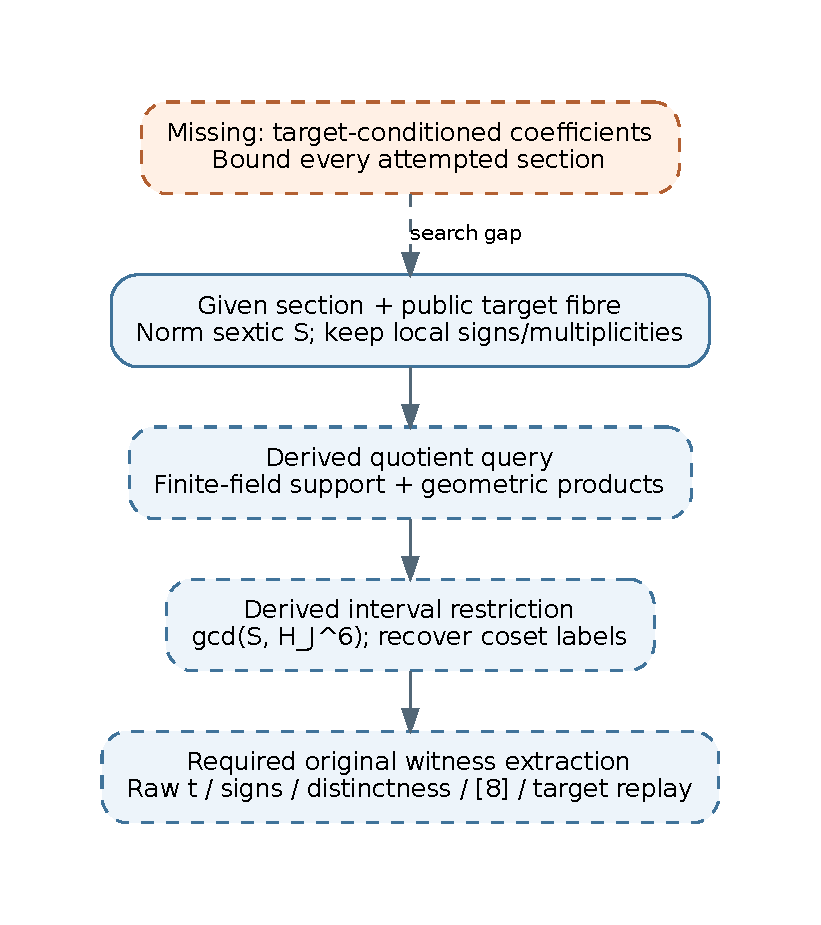
\includegraphics[height=3.6in]{flow.pdf}\end{center}
\textbf{Domain.} Original exact-order/map contracts, \(p\) odd with2 nonsquare,
\(h\) of order \(aq\), odd \(a,q\), \(q\mid p+1\), \(2k<a\), and full target-fibre
coverage. Every returned row still needs original raw-index, sign,
distinctness, nonidentity-image and public-target checks. No chart refusal
is target absence. Classical section/norm theory is prior art [1,2,5].

\newpage
\begin{center}{\Large\bfseries Query and restriction recurrence}\end{center}
In \(\mathcal A=\mathbb F_p[X]/S\), of dimension6, require \(2X+A\) a unit and put
\(\lambda=A/(2X+A)\), \(u=T_q(\lambda)\), \(a_j=\Re((h^q)^j)\).
Support is tested by the three exact remainders
\[
(X^p-X)^6=0,\quad (C^{(p-1)/2}-1)^6=0,\quad
H^6=0,\qquad H=\prod_{j=1}^k(u^2-a_j^2).
\]
Sixth powers retain multiplicities: for degree6 \(S\), support containment in
the zeros of \(F\) is equivalent to \(S\mid F^6\). These tests do not replace
local sign recovery or original-row replay.

Adjoin \(v\) over \(\mathcal A\otimes\mathbb F_{p^2}\) with
\(v^2-(4u^2-2)v+1=0\). This monic algebra is free, including for repeated
roots of \(S\). The element \(v\) is a unit. For \(\rho=(h^q)^2\),
\begin{align*}
(v-\rho^j)(v-\rho^{-j})&=4v(u^2-a_j^2),\\
P_J(v;\rho)P_J(v;\rho^{-1})&=(4v)^{|J|}H_J.
\end{align*}
No factor \(v-\rho^j\) is inverted. Scalar-unit chirp operations from
geometric-product Algorithm2 [3] transfer explicitly to this fixed-dimensional
algebra; it is not treated as a field.

For \(n=s^2\), construct \(A(Z)=\prod_{j=0}^{s-1}(t-\rho^jZ)\) by homothety,
evaluate at \(1,\rho^s,\ldots,\rho^{(s-1)s}\) by chirp convolution, then multiply
the \(s\) results. Non-square tails have \(O(\sqrt n)\) factors. Interval
offsets use known scalar powers. The cost is
\[
O\bigl(M(\sqrt n)+\sqrt n\bigr)
\]
algebra operations, including scalar work and construction [3,4].
Quasi-linear polynomial multiplication gives the conditional
\(\softO(\sqrt k+\log p+\log q)\) supplied-section query bound. Naive
convolution would give linear work in \(k\).

Recover \(H_J\) by the unit \((4v)^{-|J|}\), project and check other free-basis
components vanish. Restrict with \(G_J=\gcd(S,H_J^6)\), descending only occupied
intervals. At most6 occupied paths yield \(\softO(\sqrt k)\) label-restriction
work. Factor only degree-at-most6 polynomials; recover local signed sections,
the original guarded torus lift, and raw \(t\) by the original bounded decoder.
Decoder setup and up to \(\softO(\sqrt q)\) query work remain charged.

\textbf{Checks at their scope.} Native records \texttt{IDC1h5aa2ca2649f9d3c6}
(degree3) and \texttt{IDC1ha8ad4123fd0897a8} (degree5) each passed32+32 fixed
evaluations and a plus-one refusal over \(2^{61}-1\). Nine maintained identity
module tests, fmt, strict Clippy and build pass. The maintained standalone
Lean gate passed one unit-cancellation endpoint, with propext and no
failing/trusted-native declarations. It is not the full geometric, algorithmic
or counting theorem. These checks are unsigned producer evidence.

\newpage
\begin{center}{\Large\bfseries Seed selection is the remaining search problem}\end{center}
For all attempted coefficients \(C_{\rm seed}\) and useful rows \(R_{\rm out}\),
the conditional cold contract is
\begin{align*}
W={}&W_{\rm setup}
 +C_{\rm seed}\softO(\sqrt k+\log p+\log q)\\
&+R_{\rm out}\softO(\sqrt k+\sqrt q+\log p)
 +W_{\rm private}+W_{\rm kernel}+W_{\rm recovery}.
\end{align*}
Count failed tests, scalar work, factorization's stated expected finite-field
cost, scratch space, tables and all retained rows. In a declared growing family
\(B\sim qk\), \(k=B^\theta\), \(C_{\rm seed}=B^\chi\), the testing phase needs
\(\chi+\theta/2<3\). No suitable constructor, family or useful-yield theorem
has been established.

\textbf{Scoped counting rejection.} The normalized chart \(c_4=1\) has \(p^5\)
seeds. A useful degree6 zero divisor determines its section up to scale:
two sections with that divisor have constant ratio on the projective integral
curve. For \(M\) signed preimage points there are at most
\(\binom{M+5}{6}\) degree6 divisors, allowing repeats. Therefore
\[
\Pr[\text{uniform seed is useful}]
 \le \frac{\binom{M+5}{6}}{p^5}=O(p^{-4})
 \quad\text{when }M=O(p^{1/6}).
\]
Uniform chart sampling cannot meet the stated cost model even with a cheap
membership oracle. This derived rejection is restricted to that seed
distribution and divisor model. It does not reject biased coefficient
generation, algebraic elimination, other bases or index calculus.
The actual divisor/counting Lean bridge and independent verification remain
open; no typical-target experiment is claimed.

\textbf{Next technical action.} Implement the finite-free-algebra product,
interval restriction and original lifting in separately qualified Rust; compare
exact direct remainders on fixed controls, including nonreduced quotients.
Then supply a target-conditioned biased constructor and bound every trial,
failure, useful row, private tag, kernel/recovery cost and memory term.
No solver campaign, paid run or benchmark is scheduled here.

\textbf{Provenance.} Protocol/derivation/source record c9c89b; native record
e20e6b. Source9/compiled5/archive17104bytes and retained binary match pre/post.
First build/Clippy/PATH/binder attempts remain archived. The final native
launch used a Python file-capture subprocess wrapper, a disclosed procedural
departure; arithmetic stayed in Rust, shell reproduction is supplied and no
rerun conceals the record. The old source, criteria, reports and evidence
remain frozen. No measured scoreboard row or established route edge changes.

{\small
[1] Cheng, \url{https://arxiv.org/abs/cs/0507026}, section2.
[2] Li--Wan--Zhang, \url{https://arxiv.org/abs/1501.01138}, section4.
[3] Bostan--Yurkevich, \url{https://arxiv.org/abs/2012.08656}, section2.1.
[4] Bostan--Schost, Journal of Complexity21(2005),420--446, section5.
[5] Project RR9 norm protocol, immutable commit cdbf32ff70d6560f2d5928f644b613e8f72bf7b4.
KB unavailable; exact primary-source scope and reuse are in SOURCES.md.
No novelty claim follows from the bounded review.}
\end{document}
